\documentclass[12pt]{article}

\usepackage{amsmath,amsthm,amssymb,amscd,epsfig,url}
\usepackage{fullpage}
\usepackage{times}
\usepackage{mathdots}
\newtheorem{theorem}{Theorem}[section]
\newtheorem{lemma}[theorem]{Lemma}
\newtheorem{proposition}[theorem]{Proposition}
\newtheorem{corollary}[theorem]{Corollary}
\newtheorem{conjecture}[theorem]{Conjecture}
\newtheorem{definition}[theorem]{Definition}
\newtheorem{example}[theorem]{Example}
\newtheorem{remark}[theorem]{Remark}

\usepackage{xcolor}
\usepackage{tikz}
\usetikzlibrary{arrows.meta, automata, positioning}

\def\ZZ{{\mathbb Z}}
\def\QQ{{\mathbb Q}}
\def\RR{{\mathbb R}}
\def\TT{{\mathcal{C} T}}
\def\KK{{\mathcal{C} K}}
\newcommand{\hus}{\hfill\break}
\newcommand{\bull}{\textbullet\;\;}
\def\iso{{\operatorname{\ \approx \ }}}   % isomorphism
\def\im{{\operatorname{im}}}              % image
\def\Hom{{\operatorname{Hom}}}           % homomorphisms
\def\line{{\operatorname{line} \,}}       % line graph
\def\sd{{\operatorname{sd \,}}}           % first edge subdivision graph
\def\coker{{\operatorname{coker}}}        % cokernel
\def\lcm{{\operatorname{lcm}}}             % least common multiple
\newcommand{\gcdd}{\gamma}              
\def\del{{\partial}}                      % signed incidence matrix
\def\<{{\langle}} \def\>{{\rangle}}       % Inner product
\def\ZC{{Z^\#}}                           % cycle space
\setlength{\textheight}{9in}               
%\setlength{\textwidth}{6in}               % width of text
%\setlength{\oddsidemargin}{0in}           % odd page left margin
%\setlength{\evensidemargin}{0in}          % even page left margin 

\title{Problem Set 4}
\author{CMSC 27230: Honors Theory of Algorithms}
\date{Assigned January 30, 2026, Due February 16, 2026}

\begin{document}
\maketitle

\thispagestyle{empty}
\section*{Problem 0: Collaborators and Outside Sources}
Who were your collaborators (if any)? Which outside sources (if any) did you use?
\section*{Problem 1: Bellman-Ford (20 points)}
\begin{enumerate}
\item[(a)] 15 points: Run the Bellman-Ford algorithm on the following graph. For your answer, for each $k$ and each vertex $v \in V(G)$, you should provide the length of the shortest walk from $s$ to $v$ which uses at most $k$ edges. You may stop when $k = 11$ or the answers for $k$ are the same as the answers for $k-1$.

    \begin{center}
    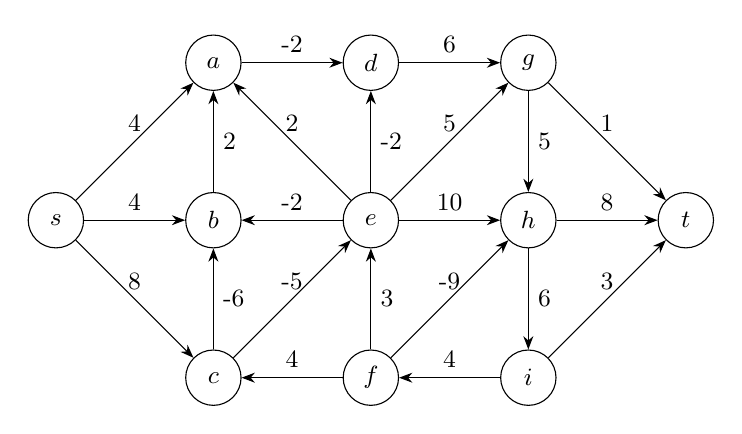
\begin{tikzpicture}[
      mycircle/.style={
         circle,
         draw=black,
         fill=white,
         fill opacity = 0.3,
         text opacity=1,
         inner sep=0pt,
         minimum size=20pt,
         font=\small},
      myarrow/.style={-Stealth},
      node distance=0.6cm and 1.2cm
      ]
      \node[mycircle]  at (-3, 0) (s) {$s$};
      \node[mycircle]  at (-1, 2) (a) {$a$};
      \node[mycircle]  at (1, 2) (d) {$d$};
      \node[mycircle]  at (-1, 0) (b) {$b$};
      \node[mycircle]  at (1, 0) (e) {$e$};
      \node[mycircle]  at (-1, -2) (c) {$c$};
      \node[mycircle]  at (1, -2) (f) {$f$};
      \node[mycircle]  at (3, 2) (g) {$g$};
      \node[mycircle]  at (3, 0) (h) {$h$};
      \node[mycircle]  at (3, -2) (i) {$i$};
      \node[mycircle]  at (5, 0) (t) {$t$};

    \foreach \i/\j/\txt/\p/\pp in {% start node/end node/text/position
      s.45/a.225/4/above/0.5,
      s.00/b.180/4/above/0.5,
      s.315/c.135/8/above/0.5,
      a.00/d.180/-2/above/0.5,
      b.90/a.270/2/right/0.5,
      c.90/b.270/-6/right/0.5,
      c.45/e.225/-5/above/0.5,
      d.0/g.180/6/above/0.5,
      e.135/a.315/2/above/0.5,
      e.180/b.0/-2/above/0.5,
      e.90/d.270/-2/right/0.5,
      e.45/g.225/5/above/0.5,
      e.0/h.180/10/above/0.5,
      f.180/c.0/4/above/0.5,
      f.90/e.270/3/right/0.5,
      f.45/h.225/-9/above/0.5,
      g.270/h.90/5/right/0.5,
      g.315/t.135/1/above/0.5,
      h.00/t.180/8/above/0.5,
      h.270/i.90/6/right/0.5,
      i.180/f.0/4/above/0.5,
      i.45/t.225/3/above/0.5
      }
       \draw [myarrow] (\i) -- node[font=\small,\p,pos=\pp] {\txt} (\j);

    \end{tikzpicture}
    \end{center}
What are the shortest path(s) from $s$ to $t$?
\item[(b)] 5 points: Now let's say the length of the edge $(h,i)$ is decreased from $6$ to $4$. What would happen if we ran the Bellman-Ford algorithm on this modified graph?
\end{enumerate}
\section*{Problem 2: Road Trip Planning (25 points)}
Let's say that your are planning a road trip along a single long road which goes from $x = 0$ to $x = L$. Along this road, there are $n$ destinations where each destination has a location $x_i \in (0,L)$ and a happiness value $h_i$ for how much you will enjoy staying there. Each day, you plan to drive to a new destination and stay there for the rest of the day. However, you have limited time so you want to start at $x = 0$ at the beginning of the first day and end at $x = L$ on day $k+1$ (so that you visit exactly $k$ destinations). Moreover, you do not want to drive more than $300$ miles per day and you never want to go backwards or stay in the same location for more than one day. 

Can you plan an optimal road trip given these constraints? More precisely, can you find a schedule $S = (i_1,\ldots,i_k)$ such that \begin{enumerate}
\item $x_{i_1} \leq 300$. 
\item For all $j \in [k-1]$, $x_{i_j} < x_{i_{j+1}} \leq x_{i_j} + 300$.
\item $x_{i_{k}} \geq L - 300$.
\end{enumerate}
and $\sum_{j = 1}^{k}{h_{i_j}}$ is maximized?

Note: For this problem, you may assume that $0 < x_1 < x_2 < \ldots < x_n < L$.
\begin{enumerate}
\item[(a)] 10 points: Give a polynomial time algorithm for finding an optimal schedule $S$.
\item[(b)] 10 points: Give a rigorous proof that the recurrence relation in your algorithm is correct.
\item[(c)] 5 points: Analyze the runtime of your algorithm.
\end{enumerate}
\section*{Problem 3: Lazy Interval Scheduling (30 points)}
Consider the following variant of the weighted interval scheduling problem. There are $n$ available jobs, each of which has an interval $[a_i,b_i]$ when it must be done (if it is taken) and a weight $w_i$ which represents how much work it is to do. You are lazy, so you would like to do as little total work as possible. However, for each job $i$ that you do not take, you must have an excuse for not taking it, i.e. another job $j$ which you do take such that $(a_i,b_i) \cap (a_j,b_j) \neq \emptyset$, as otherwise your boss will see that you are available for job $i$ and make you take it (or another job you could take). Also, each job demands your full attention so you are not allowed to take two overlapping jobs. 

Can you find a schedule which satisfies these constraints and minimizes your total work? More precisely, can you find a set $S \subseteq [n]$ of jobs to take such that 
\begin{enumerate}
\item For all distinct $i,j \in S$, $(a_i,b_i) \cap (a_j,b_j) = \emptyset$.
\item For all $j \notin S$, there exists an $i \in S$ such that $(a_i,b_i) \cap (a_j,b_j) \neq \emptyset$.
\end{enumerate}
and the total work $\sum_{i \in S}{w_i}$ is as small as possible?

For example, if there are $5$ jobs with the following intervals and weights
\begin{enumerate}
\item $[a_1,b_1] = [2,4]$ and $w_1 = 4$
\item $[a_2,b_2] = [3,6]$ and $w_2 = 6$ 
\item $[a_3,b_3] = [5,8]$ and $w_3 = 3$ 
\item $[a_4,b_4] = [7,11]$ and $w_4 = 5$ 
\item $[a_5,b_5] = [10,12]$ and $w_5 = 2$ 
\end{enumerate}
then it is best to take jobs $2$ and $5$ which gives a total work of $8$.

Note: For this problem, you may assume that all of the times $a_1,\ldots,a_n,b_1,\ldots,b_n$ are distinct.
\begin{enumerate}
\item[(a)] 5 points: Your friend proposes the following greedy algorithm for the special case of the problem where $w_i = 1$ for all $i \in [n]$ (so you just want to take as few jobs as possible):

At each step, consider the job $i$ which ends earliest among all of the jobs starting after your current end time. Take the job $j$ which ends latest among all of the jobs which start after your current end time but before job $i$ ends.

More precisely, the algorithm is as follows:
\begin{enumerate}
\item[] Preprocessing: Order the jobs by both their start and end time.
\item[] Initialization: Set $S = \emptyset$, $t = min_{i \in [n]}{\{a_i\}}$.
\item[] Iterative step: Go through the array of jobs sorted by their end time and take the first job $i$ such that $a_i \geq t$. Then go through the jobs sorted by their start time and find the job $j$ such that $t \leq a_j < b_i$ and $b_j$ is maximized (note that we can have $j = i$). Add $j$ to $S$ and set $t = b_j$.
\end{enumerate}
Is this greedy algorithm correct? If so, explain why. If not, give a counterexample.
\item[(b)] 10 points: Now consider the problem with arbitrary weights. Give a polynomial time algorithm for finding an optimal schedule $S$. Hint is available.
\item[(c)] 10 points: Give a rigorous proof that the recurrence relation in your algorithm is correct.
\item[(d)] 5 points: Analyze the runtime of your algorithm.
\end{enumerate}
\section*{Problem 4: Pok\'{e}mon Battle (25 points)}
Acknowledgement: This problem is due to Andy Drucker:\\
You are an up-and-coming Pok\'{e}mon trainer supervising a training battle. Your $n$ Pok\'{e}mon $p_1, \ldots , p_n$ are arranged in a line, in that order. At each time step, a single pair of adjacent Pok\'{e}mon fight. The winner stays in battle at the same position on the line; the loser ``faints'' and is removed. The battle ends when there is only a single Pok\'{e}mon left.

As the trainer, you know for each pair $p_i, p_j$ which of the two Pok\'emon would win in a fight. This is recorded in the $(i,j)$-entry of a matrix $M$ which you can access. Still, there are many possible ways the battle could unfold, depending on which adjacent pair of Pok\'{e}mon fights next at each step.

\begin{example}
A special case of this problem is as follows. There are water Pok\'{e}mon, fire Pok\'{e}mon, and grass Pok\'{e}mon and each Pok\'{e}mon has a level. Water Pok\'{e}mon defeat all fire Pok\'{e}mon as well as water Pok\'{e}mon of lower level. Fire Pok\'{e}mon defeat all grass Pok\'{e}mon as well as fire Pok\'{e}mon of lower level. Grass Pok\'{e}mon defeat all water Pok\'{e}mon as well as grass Pok\'{e}mon of lower level.

If the lineup is $W1,F1,G1$ (where $F$, $W$, and $G$ stand for fire, water, and grass respectively and the number gives the level) then the $W1$ and $G1$ Pok\'{e}mon can win but the $F1$ Pok\'{e}mon cannot win. To see this, observe that
\begin{enumerate}
\item If we first have $F1$ and $G1$ fight then $F1$ will win. $W1$ will then fight $F1$ and win.
\item If we first have $W1$ and $F1$ fight then $W1$ will win. $G1$ will then fight $W1$ and win.
\end{enumerate}

If we instead have the lineup $G2,F1,W1,G1$ then every Pok\'{e}mon except $W1$ can win. To see this, observe that 
\begin{enumerate}
\item If we first have $F1$ and $W1$ fight then $W1$ will win. $W1$ will then fight $G1$ or $G2$ and lose. $G2$ will then fight $G1$ and win.
\item If we first have $W1$ and $G1$ fight then $G1$ will win. $F1$ will then fight $G1$ and $G2$ (in either order) and win both fights.
\item If we first have $G2$ and $F1$ fight then $F1$ will win. If we then have $W1$ and $F1$ fight then $W1$ will win. $G1$ will then fight $W1$ and win.
\item $W1$ cannot win the battle as if $W1$ is not defeated by $G2$ then $W1$ will have to fight $G1$.
\end{enumerate}
\end{example}
\begin{enumerate}
\item[(a)] 10 points: Give a polynomial time algorithm that outputs a list of all possible winners of the battle. Hint is available.
\item[(b)] 10 points: Explain why your algorithm is correct. You do not need to give a rigorous proof.
\item[(c)] 5 points: Analyze the runtime of your algorithm.
\end{enumerate}
\newpage
\section*{Hints}
\noindent 3a. It may help to find a set of jobs such that you must take at least one job from this set and then determine the best you can do by taking each job in this set. Remember to specify the order for solving the subproblems.\\
\\
4a. You should solve the following subproblems. For each interval $[l,r]$, which Pok\'{e}mon could win the battle between Pok\'{e}mon $p_l,\ldots,p_r$? Remember to specify the order for solving the subproblems.

\end{document}
